\documentclass[11pt,letterpaper]{article}
\usepackage{anysize}
\usepackage{indentfirst}
\usepackage{sectsty}
\usepackage{amsmath}
\usepackage{hyperref}
\usepackage{graphicx}
\usepackage{chngpage}
\usepackage{enumerate}
\hypersetup{
	colorlinks=true, 
	linkcolor=blue, 
	urlcolor=blue, 
	pdfnewwindow=true, 
	citecolor=black
}
\urlstyle{same}
\linespread{1.2}

\begin{document}

\begin{titlepage}
    \vspace*{4cm}
    \begin{flushright}
    {\huge
        Project 1\\[5mm]
    }
    {\large
        CS325 | Spring 2015
     }
    \end{flushright}
\hrule
    \begin{flushright}
	by Group 2\\
	Vedanth Narayanan\\
	Jonathan Merrill\\
	Tracie Lee\\
    \vfill
	\today\\
    \end{flushright}
\end{titlepage}

\raggedright

\section{Theoretical Run-time Analysis}

\subsection{Algorithm 1}
\begin{verbatim}
    maxSubarray(a[1,...,n])
        max = a[0]
        for i = [0...n]
            for j = [i,n]
                sum = 0
                for each pair(i,j) with 1<=i<=j<=n
        	        compute a[i]+a[j+1]+...+a[j-1]+a[j]
            keep max sum found so far
        return max sum found
\end{verbatim}
\textbf{Asymptotic Analysis}\\
We have $O(n^2)$ pairs * $O(n)$ time to compute each sum $= O(n^3)$.

\subsection{Algorithm 2}
\begin{verbatim}
    maxSubarray(a[1,...,n])
        for i = 1, ...., n
            sum = 0
            for = i, ...., n
                sum = sum + a[j]
                keep max sum found so far
        return max sum found
\end{verbatim}
\textbf{Asymptotic Analysis}\\
We have $O(n)$ i-iterations (outer loop) * $O(n)$ j-iterations (inner loop) * $O(n)$ for the time to update $= O(n^2)$.

\subsection{Algorithm 3}
\begin{verbatim}
    maxSubarray(a[1,...,n], initial array length)
        length = len(a)

        if length > 1:
            left = left half of array
            right = right half of array
            first = maxSubarray(left, 0)
            last = maxSubarray(right, 0)
            reverse left
            center = helper(left) + helper(right)
        else:
            first = last = center = a[0]

        if initial array length == len(a):
            PrintResults(max([first, last, center]), a, [first, last, center])

        return max([first, last, center])

    helper(a):
        max = a[0]
        sum = 0
        for i in range(0, len(a)):
            sum += a[i]
            if sum > max:
                max = sum
        return max
\end{verbatim}
\textbf{Asymptotic Analysis}\\
We have $T(n) = 2T(\frac{n}{2}) + \Theta(n)$. This falls within Case 2 of the Master Method, and therefore yields a solution of $\Theta(nlgn)$.

\subsection{Algorithm 4}
\begin{verbatim}
    maxSubarray(a[1,...,n])

    maybeStart = 0
    start = 0
    end = 0
    i = a[0]
    sum = a[0]
    small = minimum of (0, i)

    for j in range(1,len(a)):
        i = i + a[j]
        if (i - small) > sum:
            start = maybeStart
            end = j+1
            sum = (i - small)
        if i < small:
            maybeStart = j+1
            small = i
    return (sum, a, a[start:end])
\end{verbatim}
\textbf{Asymptotic Analysis}\\
We have $O(n)$ things to compute, therefore this takes $O(n)$ time.


\section{Proof of Correctness: Algorithm 3}
\subsection*{Base Case}
We pass in either an empty array or an array consisting of 1 element. In the first case, an empty array is returned and in the second case the algorithm returns the same array that had been passed in since it is the max subarray within that array.

\subsection*{Inductive Hypothesis}
Assume that algorithm 3 correctly returns a maximum contiguous sum of elements $s$ from an array $A$ of $n > 1$ elements. 

\subsection*{Inductive Step}
If we split $A$ into 2 separate arrays, let $L$ represent the new array from the left side and let $R$ represent the new array from the right side. Then let $s_{i...j}$ represent any sequence of numbers with the largest sum that lies with in $S$. If the sum of $s_{i...j} = x$, then $max(first, last, center) \leq x$. There are then 3 possibilities:
\begin{enumerate}
\item $s_{i...j}$ lies completely within $L$. In this case, it would follow that the max subarray of $L$ is equal to x which means that $max(first, last, center) \geq first = x$. Because of this, we know that the answer returned is exactly x.
\item $s_{i...j}$ lies completely within $R$. In this case, it would follow that the max subarray of $R$ is equal to x which means that $max(first, last, center) \geq last = x$. Because of this, we know that the answer returned is exactly x.
\item If $s_{i...j}$ does not lie completely within $L$ or $R$, then it must start in $L$ and end in $R$. 
\end{enumerate}

\section{Testing}
\centerline{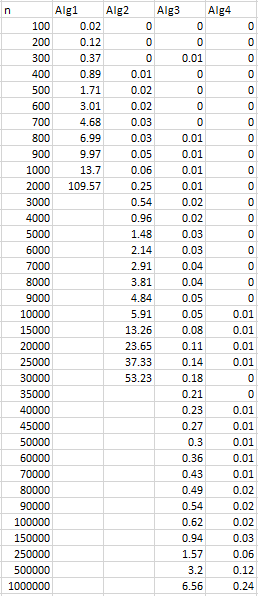
\includegraphics[width=3in]{TestTimes.png}}

\pagebreak
\section{Experimental Analysis}
\centerline{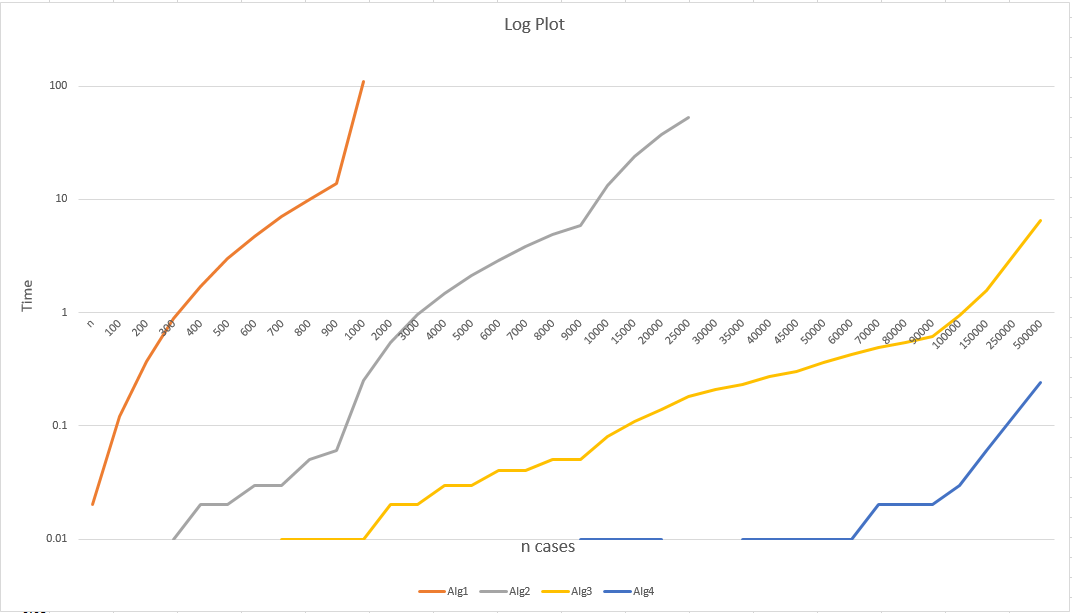
\includegraphics[width=7in]{LogPlot.png}}

\section{Extrapolation and Interpretation}
In general, our test data confirmed that our asymptotic analysis for each algorithm was very close. Algorithm was predicted to be $O(n^3)$, algorithm 2 $O(n^2)$, algorithm 3 $O(nlgn)$ and algorithm 4 $O(n)$, and all 4 algorithm plots have curves that are roughly equivalent.\vspace{8pt}
\\
To find the largest instance that can be solved within an hour for each algorithm, we had to do some rough estimating. Assuming that algorithm 1 is indeed $O(n^3)$, we used our largest testing trial for algorithm 1 ($n=2000$; completing in 109 seconds) to find the approximate number of operations the computer can do each second:\vspace{8pt}
\\
\hspace{10mm}$2000^3 / 109 = 73394495$ operations per second\vspace{8pt}
\\
Then, using the complexities we found for each algorithm, we could solve for n using a time restraint of one hour,  and the operations per second found above:\\
\begin{itemize}
\item Algorithm 1: $n=6400$
\item Algorithm 2: $n=514023$
\item Algorithm 3: $n=8.02*10^9$
\item Algorithm 4: $n=2.64*10^{11}$
\end{itemize}

\end{document}
